%! Tex program = pdflatex
 
\documentclass[UTF8]{ctexart}
\CTEXsetup[format={\Large\bfseries}]{section}
\usepackage{amsmath}
\usepackage{ctex}
\usepackage{array}
\usepackage{ulem}
\usepackage{graphicx}
\usepackage{geometry}
\usepackage{multirow}
\usepackage{subfig}
\usepackage{float}
\usepackage{multicol}
\usepackage{multirow}
\usepackage{indentfirst}
\usepackage{makecell}
\geometry{papersize={21cm,29.7cm}}
\geometry{left=2.54cm,right=2.54cm,top=3.18cm,bottom=3.18cm}
\usepackage{fancyhdr}
\pagestyle{fancy}
\lhead{\today}
\chead{}
\rhead{2020011075}
\lfoot{清华大学}
\cfoot{\thepage}
\rfoot{系统工程导论}
\renewcommand{\headrulewidth}{0.4pt}
\renewcommand{\headwidth}{\textwidth}
\renewcommand{\footrulewidth}{0pt}
\usepackage{bm}

\begin{document}

\begin{center}
  \Large{系统工程导论作业二——系统建模}\\
\end{center}
\begin{center}
  \large{彭程 2020011075}
\end{center}
\section{题目一}
\subsection{用分块矩阵方法确定可达矩阵R 对应变量的骨架图,写出详细过程;}

\noindent 解:

对于可达矩阵R,记变量依次为  1,2,3,4,5,6,7 

$$
R=\left[\begin{array}{lllllll}
1 & 1 & 0 & 0 & 1 & 0 & 1 \\
0 & 1 & 0 & 0 & 0 & 0 & 1 \\
0 & 0 & 1 & 1 & 1 & 0 & 1 \\
0 & 0 & 1 & 1 & 1 & 0 & 1 \\
0 & 0 & 0 & 0 & 1 & 0 & 1 \\
1 & 1 & 1 & 1 & 1 & 1 & 1 \\
0 & 0 & 0 & 0 & 0 & 0 & 1
\end{array}\right]
$$



\noindent (1)选择参考变量 1;

\noindent (2)将其他元素和1比较有:

\begin{align}
A(1)&=\{2,5,7\} \nonumber\\
B(1)&=\{\} \nonumber\\
C(1)&=\{3,4\} \nonumber\\
D(1)&=\{6\}\nonumber
\end{align}

\noindent (3)分析对角块:

分块矩阵为:
$$
\begin{matrix}
  \begin{matrix}~~~~~~A~&~~B&~1&~~C~&~~~D\\
\end{matrix}&\ \\
R=\left[
  \begin{matrix}
    M_{AA}&0&0&0&0\\
    1&1&1&0&0\\
    1&1&1&0&0\\
    M_{CA}&0&0&M_{CC}&0\\
    1&1&1&M_{DC}&M_{DD}\\
  \end{matrix}
  \right]
  &\begin{matrix}A\\B\\1\\C\\D\\\end{matrix}\\\end{matrix}
$$

初步骨架图为:

\begin{figure}[H]
  \centering
  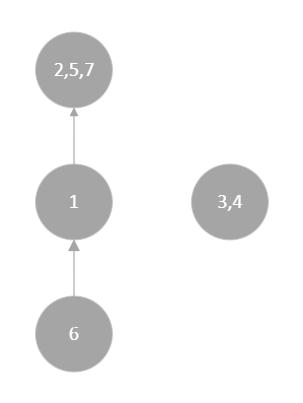
\includegraphics[scale=0.8]{1.png}
\end{figure}

接下来考察$M_{AA},M_{CC}$:
$$
\begin{matrix}\begin{matrix}~~~~~~~~~~~~2&5&7\\\end{matrix}&\ \\M_{AA}=\left[\begin{matrix}1&0&1\\0&1&1\\0&0&1\\\end{matrix}\right]&\begin{matrix}2\\5\\7\\\end{matrix}\\\end{matrix}
$$

骨架图为:

\begin{figure}[H]
  \centering
  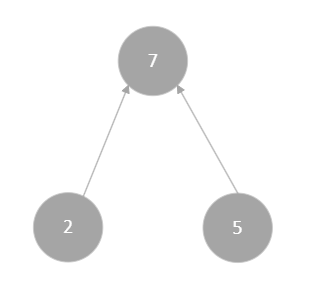
\includegraphics[scale=0.8]{2.png}
\end{figure}

$$
\begin{matrix}\begin{matrix}~~~~~~~~~~~~3&4\\\end{matrix}&\ \\M_{CC}=\left[\begin{matrix}1&1\\1&1\\\end{matrix}\right]&\begin{matrix}3\\4\\\end{matrix}\\\end{matrix}
$$

骨架图为:

\begin{figure}[H]
  \centering
  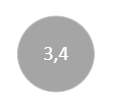
\includegraphics[scale=0.8]{3.png}
\end{figure}

汇总得到:

\begin{figure}[H]
  \centering
  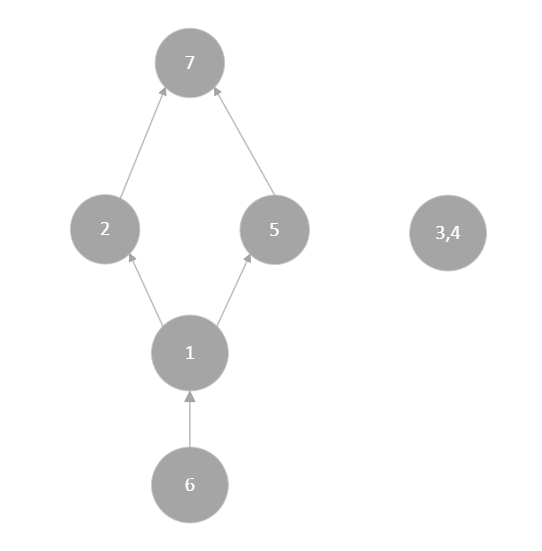
\includegraphics[scale=0.8]{4.png}
\end{figure}

接下来考察3、4和2、5、7的关系,发现3、4可达5但不可达2,6可达3、4,故最终骨架图如下:

\begin{figure}[H]
  \centering
  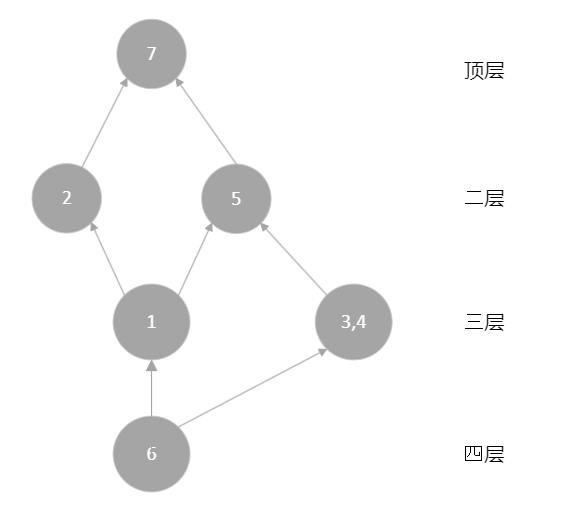
\includegraphics[scale=0.8]{5.png}
\end{figure}

\subsection{写出下图所示骨架图的邻接矩阵,计算出图中所有恰好2度可达的路径,并列
举出来(路径格式示例: 1->2->3)。}

\begin{figure}[H]
  \centering
  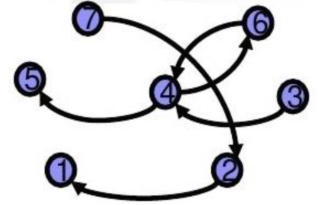
\includegraphics[scale=1]{6.png}
\end{figure}

\noindent 解:

邻接矩阵为:

$$
A=\left[\begin{matrix}0&0&0&0&0&0&0\\1&0&0&0&0&0&0\\0&0&0&1&0&0&0\\0&0&0&0&1&1&0\\0&0&0&0&0&0&0\\0&0&0&1&0&0&0\\0&1&0&0&0&0&0\\\end{matrix}\right]
$$

要求两步可达的路径则只需要求$A^2$:

$$
A^2=\left[\begin{matrix}0&0&0&0&0&0&0\\0&0&0&0&0&0&0\\0&0&0&0&1&1&0\\0&0&0&1&0&0&0\\0&0&0&0&0&0&0\\0&0&0&0&1&1&0\\1&0&0&0&0&0&0\\\end{matrix}\right]
$$

故可以得到两步可达的路径为:
$$
\begin{array}{c}
3\rightarrow 4\rightarrow 5\\
3\rightarrow 4\rightarrow 6\\
4\rightarrow 6\rightarrow 4\\
6\rightarrow 4\rightarrow 5\\
6\rightarrow 4\rightarrow 6\\
7\rightarrow 2\rightarrow 1\\
\end{array}
$$


\section{题目二}

\subsection{请你选择一门自己学过的课程,以课本章节(或者讲义章节) 为单元,运用系统
工程导论第三章所学的知识,画出这门课的知识体系骨架图}

\noindent 规定:

如果单元B中需要大量运用单元A中讲解的知识,否则难以学习,则可以确定A→B;

若两者知识点上相互独立,则AB之间无关系;

若两者都有共同的知识基础,并且在内容上也有互相呼应,则可以AB。

\noindent 解:

《数据结构》知识体系骨架图如下:


\begin{figure}[H]
  \centering
  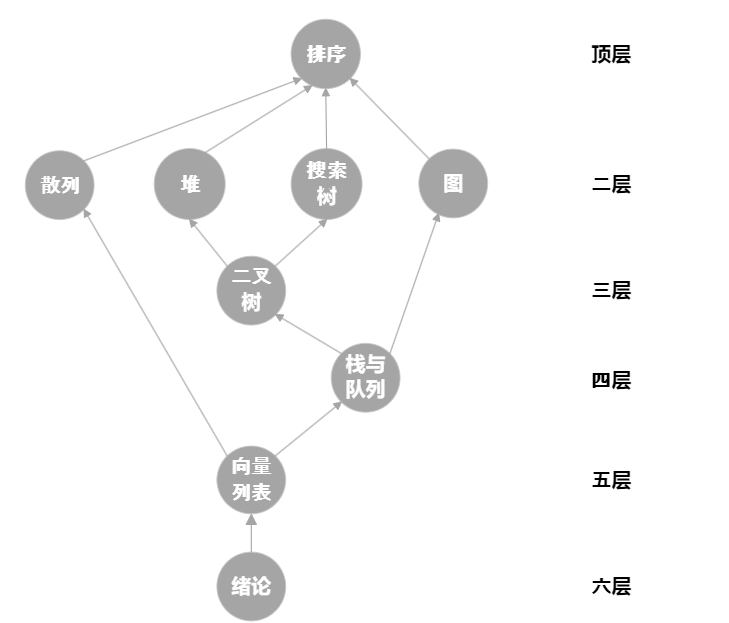
\includegraphics[scale=1]{7.png}
\end{figure}


\noindent 说明:

上图展示了《数据结构》的知识体系:首先课程绪论讲述了数据结构的基本概念和复杂度的分析方法,这是后续对于各种数据结构的分析所不可缺少的知识;然后介绍了向量与列表;此后讲到的栈与队列、散列的实现需要依靠向量和列表;二叉树和图的实现特别是其中深度、广度优先搜索算法都依靠栈与队列;搜索树和堆的实现都离不开二叉树;最后排序方法依赖于讲过的所有数据结构的性质,例如依赖于散列的桶排序、依赖于图的拓扑排序、依赖于树的快排、和依赖于堆的堆排序。


\end{document}